\documentclass[UTF8]{ctexart}
\usepackage{amsmath,amssymb}
\usepackage{tikz}
\usepackage[colorlinks]{hyperref}
\usepackage{fontawesome}
\usetikzlibrary{calendar}
\usetikzlibrary{math}
\ctexset{
    section/format += \sffamily,
    subsection/format += \sffamily,
}
\begin{document}
    \title{\sffamily Log Creative 个人主页开发}
    \author{Log Creative}
    \maketitle
    
    \begin{quotation}
        \noindent \centering \LARGE \emph{学习大前端}
    \end{quotation}
    
\section{日程安排}

    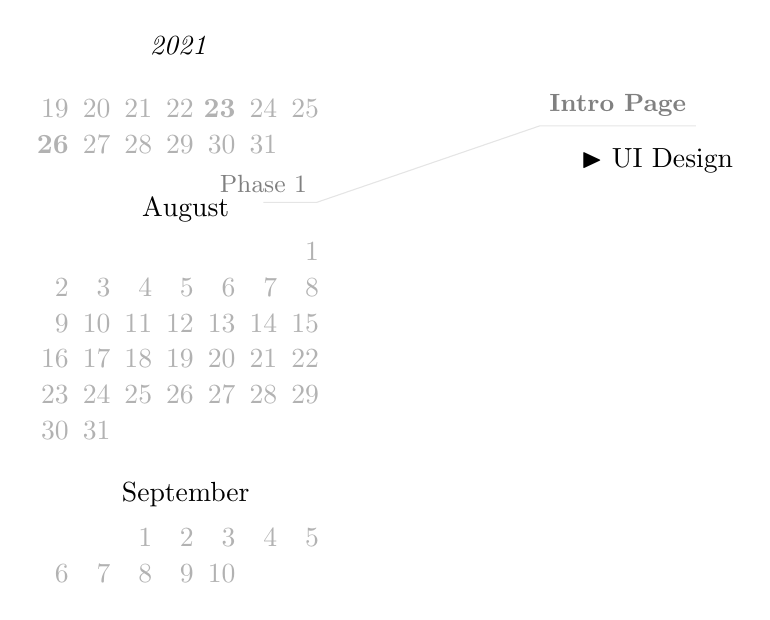
\begin{tikzpicture}[node distance=0.5cm]
        \tikzstyle{note} = [font=\small, black!50];
        \tikzstyle{content} = [note, xshift=4cm, yshift=0.5cm];
        \tikzstyle{noteline} = [black!10];
        \tikzstyle{detail} = [xshift=0.5cm,yshift=-0.2cm];
        \tikzstyle{live} = [font=\bfseries];

        \calendar (cal) [
            dates=2021-07-19 to 2021-09-10, 
            week list, 
            month label above centered
        ]   if (Saturday, Sunday) [red]
            if (at most=\year-\month-\day) [black!30]
            if (equals=\year-\month-\day) [blue]
            if (equals=2021-07-23) [live]
            if (equals=2021-07-26) [live];
        \node [above of=cal-2021-07-22, node distance=0.8cm] {\emph{2021}};

        \node [below of=cal-2021-07-31,note] (p1n) {Phase 1};
        \node [right of=cal-2021-07-31,content] (p1c) {\textbf{Intro Page}};
        \draw [noteline] (p1n.south) -- (p1n.south east) -- (p1c.south west) -- (p1c.south east);
        \node [below of=p1c,detail] {
            $\blacktriangleright$ UI Design
        };
    \end{tikzpicture}
    
    大部分工作在开学前进行,所有工作的完成不得迟于 10 月。

    \textbf{开播于 7 月 23 日(五)}。此后每周工作日三个上午 9:00 -- 11:00 直播,但是仅每周五会介绍关于该项目的新任务,视外界环境情形可能会有日程变动。

    \clearpage
\section{项目定位}

    学点前端,搞个可以营生的技能。

    前端的个人主页侧重于介绍,但是东西比较繁杂,需要一定的模块封装提高效率和可拓展性。在这个项目中尽可能多地涉及前端相关知识点,元素尽可能矢量,代码尽可能原创,这样可以显著减少文件体积以部署在 GitHub Pages 上。

    对于静态页面,本人用 \LaTeX{} 可能比网页写得更好。因此需要更好地利用网页的技术特性:动画、响应式、可交互性。内页偏向于全页浸入式风格,作为大前端,就需要自己进行一定的交互与视觉设计,并使用各种各样的软件辅助以尽可能达到预期效果。

    % 相关进度信息、关联项

\section{直播内容}

    每次直播 2 个小时,主要讨论:
    \begin{description}
        \item[UX/UI 设计] 独立项目美工靠自己!在线绘制界面草稿、交互设计稿与实现原型稿。
        \item[前端路线] 工具的选择十分重要!使用什么样的库可以更快地实现一些效果,避免重复造轮子。
        \item[中端实施] 代码赋予网页灵魂!中端是自造的词,主要是前端的 JavaScript 代码的练习以及对应的框架使用。
        \item[后端初探] 有了后端网页就有功能了!如果时间足够---以及资金足够,可以尝试加入项目数据库,配合前端进行展示。 
    \end{description}

    下播到下一次直播之前会尽量对讨论出的内容进行实施,直播过程中不会有太多的空窗时间(并尽可能多整活),直播前会做一些调研准备。

    \begin{figure}[h]
        \centering
        \begin{tikzpicture}
            \tikzstyle{fade} = [opacity=0.5];
            \def\w{2cm}
            \def\m{3}
            \def\c{1}
            \def\notice{正在准备}
            \foreach \n in {1,...,4}{
                \pgfmathparse{\n*\m}\let\x=\pgfmathresult
                \pgfmathparse{\c*25}\let\p=\pgfmathresult
                \ifx\n\c \node (s\n) at (\x,0) {\includegraphics[width=\w]{img/ProfilePhoto\n.png}};
                \node [below of=s\n, node distance=1.5cm] {\notice~\p\%};
                \else \node [fade] (s\n) at (\x,0) {\includegraphics[width=\w]{img/ProfilePhoto\n.png}};
                \fi
            }
            \draw [->] (s1) -- (s2);
            \draw [->] (s2) -- (s3);
            \draw [->] (s3) -- (s4);
        \end{tikzpicture}
    \end{figure}

\subsection*{正在进行的准备}

    在制作个人主页的同时,也会在制作过程中寻找需求,做一些其他的小工具,以更好地练习编程技能。

    修改 \href{https://gitee.com/LogCreative/obs-auto-subtitle}{obs-auto-subtitle} 项目,以更好地适配华为云自动识别。

    需要自动生成 token 的工具,可以用前端写一个,(OBS 编译太麻烦了,改的头秃)。但是发现前端有跨域访问的限制,在这一点上可能使用内嵌工具会更加方便些,至少生成了一个可用的版本。

    \noindent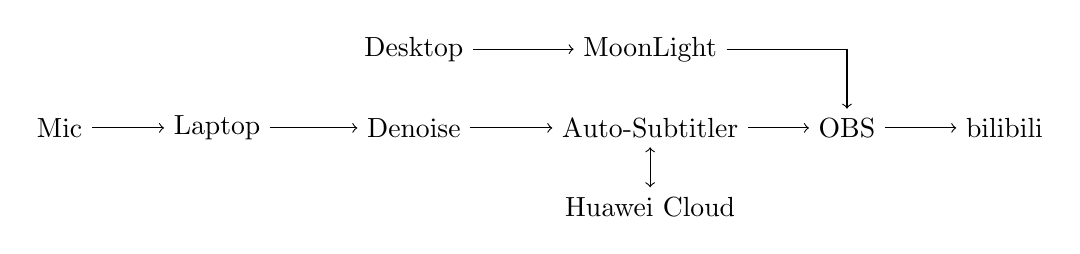
\begin{tikzpicture}
        \tikzstyle{arrow}=[->];
        \node (v1) at (-3,0) {Mic};
        \node (v2) at (-1,0) {Laptop};
        \draw [arrow] (v1) edge (v2);
        \node (v3) at (1.5,0) {Denoise};
        \node (v4) at (4.5,0) {Auto-Subtitler};
        \draw [arrow] (v2) edge (v3);
        \draw [arrow] (v3) edge (v4);
        \node (v5) at (7,0) {OBS};
        \draw [arrow] (v4) edge (v5);
        \node (v6) at (1.5,1) {Desktop};
        
        \node (v7) at (4.5,1) {MoonLight};
        \draw [arrow] (v6) edge (v7);
        
        \draw [arrow] (v7) --+(2.5,0) -| (v5);
        
        \node (v8) at (4.5,-1) {Huawei Cloud};
        \draw [<->]  (v4) edge (v8);
        \node (v9) at (9,0) {bilibili};
        \draw [arrow]  (v5) edge (v9);
    \end{tikzpicture}

    构造 \href{https://github.com/LogCreative/manim-subtitler}{manim-subtitler} 项目,以更好地向视频中添加 \LaTeX{} 字幕。

\section{目前进度}

    对内核项定名:NeuCV = Neumorphism + CV (Curriculum Vitae),创建新的存储库,使用 WTFPL 授权。

    视觉风格、总框架:渐变、拟物

    Intro Page UI: 环状发散、剪切路径

    \faYoutubePlay~\href{https://www.bilibili.com/video/BV1Lh411z7tZ/}{直播集锦}

    % 像模像样 LaTeX 第一节
    % 录制
    % 规整素材
    % LaTeX Q&A (optional)
    % CSS on HwCloudTokenGenerator
    % Design Improvement on the Intro Page

    % manim-subtitler
    % DevOps
    % 它的前端
    % Intro Page 仍然没有太好的思路

% Reference: 前端开发路线(我都不是特别会)
% 1. 网络
% (1)互联网是如何运行的?
% (2)HTTP
% (3)浏览器的工作原理
% (4)DNS(域名)
% (5)What is hosting?
% 2. HTML
% (1)HTML基础
% (2)语义化标签
% (3)表单验证
% (4)HTML最佳实践
% (5)页面可访问性(HTML accessbility)
% 3. CSS
% (1)CSS基础
% (2)布局(float、position、display、box model、Grid布局、flex box)
% (3)响应式设计与媒体查询
% 4. JavaScript
% (1)语法
% (2)DOM
% (3)fetch 和 Ajax
% (4)ES6 与 模块化JS
% (5)难点(变量提升、事件冒泡、作用域、原型链、虚拟dom、严格模式)
% 5. 版本控制
% (1)Git 操作
% (2)github项目托管(github、gitlab、bitbucket)
% 6. 网络安全
% (1)HTTPS
% (2)CORS
% (3)content security policity内容安全策略
% (4)OWASP安全风险
% 7. 包管理工具
% (1)NPM
% (2)Yarn
% 8. CSS架构
% (1)BEM(block、element、modifier)
% (2)OOCSS(面向对象的CSS)
% (3)SMACSS
% 9. CSS预处理
% (1)SCSS
% (2)PostCSS
% (3)LESS
% 10. 构建工具
% (1)npm scripts
% (2)GULP
% (3)Prettier(JS美化工具)
% (4)ESLint
% (5)StandardJS
% (6)Webpack
% (7)Rollup
% (8)Parcel
% 11. VUE
% (1)VUE基础
% (2)VUEX
% (3)VUE Router
% (4)Vue cli
% 12. React
% (1)React基础
% (2)Redux
% (3)React-Router
% (4)React Cli
% 13. 现代CSS
% (1)样式化组建(Styled Component)
% (2)Css模块(CSS Module)
% (3)Styled JSX
% (4)Emotion (CSS-in-JS)
% (5)Radium
% (6)Glamorou
% 14. Web components
% (1)HTML Templates
% (2)Custom Elements
% (3)Shadow DOM
% 15. CSS框架
% (1)Reactstrop
% (2)Material UI
% (3)Tailwind CSS
% (4)Chakra UI
% (5)Bootstrap
% (6)Materialize
% (7)Bulma
% 16. 测试
% (1)Jest
% (2)react-testing-library
% (3)Cypress
% (4)Enzyme
% 17. Mocha、Chai、Ava、Jasmine(JS测试框架)
% 18. 类型检测
% (1)TypeScript
% (2)Flow
% 19. 渐进式web应用
% (1)Storage
% (2)Web Sockets
% (3)Service Workers
% (4)Location
% (5)Notifications
% (6)Device Orientation
% (7)Payments
% (8)Credentials
% (9)PRPL Pattern
% (10)RAIL Model
% (11)Performance Metrics
% (12)Using Lighthouse
% (13)Using devTools
% 20. 服务端渲染(SSR)
% (1)VUE-SSR实践 
% (2)Nuxt.js
% (3)React SSR
% (4)NESTJS笔记、After.js
% 21. GraphQL
% (1)Apollo
% (2)Relay Modern
% 22. 静态站点
% > 11ty
% (1)GatsbyJS
% (2)Vuepress
% (3)Jekyll
% (4)Hugo
% (5)Gridsome
% 23. 移动应用
% (1)React-Native
% (2)NativeScript
% (3)Flutter
% (4)Ionic
% 24. 桌面应用
% (1)Electron
% (2)Cario
% (3)Proton Native
% 25. Web Assembly


\end{document}